\begin{Problem}
	Sei $G$ eine Gruppe mit neutralem Element 1. Für jedes Element $g \in G$ gelte $g^2 = 1$. Zeigen Sie, dass G dann abelsch ist.
\end{Problem}

\begin{proof}
\begin{Lemma}
	Sei $a,b\in G$. Dann gilt $(ab)^{-1}=b^{-1}a^{-1}$.
\end{Lemma}
\begin{proof}
	\[abb^{-1}a^{-1}=a(bb^{-1})a^{-1}=aa^{-1}=1.\qedhere\]
\end{proof}
Es gilt, f\"{u}r jede $g\in G$, dass $g=g^{-1}$, weil $gg=1$ (per Definition). Deswegen gilt
\[
ab=(ab)^{-1}=b^{-1}a^{-1}=ba
.\qedhere\] 
\end{proof}

\begin{Problem}
	Sei $K$ ein endlicher Körper mit $q \in \N^*$ Elementen.
	\begin{parts}
		\item Zeigen Sie, dass es genau $\prod_{k=0}^{n-1} (q^n-q^k)$ geordnete Basen des $K$-Vektorraums $K^n$ gibt. Unter einer geordneten Basis des $K$-Vektorraums $K^n$ verstehen wir hierbei ein n-Tupel $(b_1 , \dots, b_n)$ linear unabhängiger Vektoren $b_1, \dots, b_n \in K^n$.
		\item Nutzen Sie Teilaufgabe (a), um nachzuweisen, dass die Gruppe $GL_n(K)$ aus Beispiel 2.4 (d) die Ordnung $\prod_{k=0}^{n-1} (q^n-q^k) $ besitzt.
	\end{parts}
\end{Problem}

\begin{proof}
	\begin{parts}	
	\item Wir versuchen, ein $p$-Tupel lineare unabhängig Vektoren zu finden. Ich zeige, dass es genau $\prod_{k=0}^{p-1}\left( q^n-q^k \right)$ solche Vektoren gibt. F\"{u}r $p=n$ ist das nat\"{u}rlich die gew\"{u}nschte Behauptung.

	F\"{u}r $p=1$ müssen wir $n$ Elemente aus $K$ finden. Es gibt $q^n$ Möglichkeiten dafür. Jedoch ist $(0,0,\dots,0)$ verboten. Deswegen gibt es genau $q^n-1$ Vektoren, die nicht $(0,0,\dots,0)$ sind.

	Jetzt nehmen wir an, dass es genau $\prod_{k=0}^{p-1} \left( q^n-q^k \right)  $ Tupel von $p$ lineare unabhängig Vektoren gibt (wenn man die Reihenfolge berücksichtig), f\"{u}r eine beliebige $p<n$. Sei $v_1,v_2,\dots, v_p$ ein solches $p$-Tupel. Wir möchten eine andere Vektor  $v_{p+1}$ finden, die lineare unabhängig von $v_1,v_2,\dots, v_p$ ist. Das bedeutet:
	\[
		v_{p+1}\neq a_1v_1+a_2v_2+\dots+a_p v_p
	\] 
	f\"{u}r \textbf{alle} $a_1,a_2,\dots, a_p\in K$. Es gibt $p^q$ Kombinationen f\"{u}r $(a_1,a_2,\dots,a_p)$. Weil $v_1,v_2,\dots, v_p$ linear unabhängig sind, gilt f\"{u}r jede $(a_1,a_2,\dots, a_p)\neq (a_1',a_2',\dots, a_p')$ auch $a_1v_1+\dots+a_pv_p\neq a_1'v_1+\dots+a_p' v\dots+a_p' v_p$. Deswegen gibt es f\"{u}r jede $v_1,v_2,\dots, v_p$ genau $q^n-q^p$ Möglichkeiten für $v_{p+1}$. 

Es gibt daher
\[
\prod_{k=0}^{p-1}\left( q^n-q^k \right)   
\]
$p$-Tuple von linear unabhängig Vektoren. F\"{u}r $p=n$ ist die Behauptung bewiesen.
\item Sei $v_1,v_2,\dots, v_n$ ein Basis von $K^n$, und $T$ eine lineare Abbildung $T:K^n\to K^n$. Wenn man $T(v_1),T(v_2),\dots, T(v_n)$ weiß, ist $T$ eindeutig. $T$ is invertierbar genau wenn $T(v_1), T(v_2),\dots,T(v_n)$ linear unabhängig sind. Es gibt dadurch eine bijektive Funktion
	\[
		f:GL_n(K)\to \left\{ (v_1,v_2,\dots,v_n)\in K^{n \times n}|v_1,\dots, v_n\text{ sind linear unabhängig} \right\} 
	.\] 
	Aber wir wissen, dass es genau $\prod_{k=0}^{n-1} \left( q^n-q^k \right)  $ solche $(v_1,v_2,\dots,v_n)\in K^{n \times n}$ gibt. Daraus folgt:
	\[
	\left|GL_n(K)\right|=\prod_{k=0}^{n-1} \left( q^n-q^k \right)  
	.\qedhere\] 
	\end{parts}
\end{proof}
\begin{Problem}
	Wir betrachten die komplexen $(2 \times  2)$-Matrizen
	\[
		E:=\begin{pmatrix} 1 & 0 \\ 0 & 1 \end{pmatrix} \qquad I:=\begin{pmatrix} i & 0 \\ 0 & -i \end{pmatrix} \qquad J:=\begin{pmatrix} 0 & 1 \\ -1 & 0 \end{pmatrix} \qquad K:=\begin{pmatrix} 0 & i \\ i & 0 \end{pmatrix} 
	.\] 
	Zeigen Sie, dass die Menge $Q_8 := \{\pm E, \pm I, \pm J, \pm K\}$ zusammen mit der Matrixmultiplikation eine nicht-abelsche Gruppe der Ordnung 8 bildet. Man nennt $Q_8$ auch die \emph{Quaternionengruppe} der Ordnung 8.

	\textbf{Hinweis:}  Ein paar konkrete Matrixmultiplikationen werden Sie bei dieser Aufgabe ausrechnen müssen. Versuchen Sie, deren Anzahl gering zu halten und möglichst viel aus Ihren bereits durchgeführten Rechnungen zu schließen.
\end{Problem}
\begin{proof}
	Wir zeigen zuerst, dass $Q_8$ under $\cdot$ abgeschlossen ist. Wir wissen von der Linearen Algebra, dass $EM=M$ f\"{u}r alle Matrizen $M$. Das heißt, dass $E$ ein neutrales Element ist. Wir wissen auch, dass $(-E)M=-M$. Ich betrachte einige wichtige Matrixmultiplikationen:
	\[
	I^2=J^2=K^2=-E
	.\]
	Daraus folgt, dass $x^{-1}=-x$, f\"{u}r $Q_8\ni x \neq \pm E$. F\"{u}r $x=-E$ ist $x^{-1}=x$. Jede $x\in G$ ist daher invertierbar.
	Es gilt auch
	\begin{align*}
		IJ=&\begin{pmatrix} i & 0 \\ 0 & -i \end{pmatrix} \begin{pmatrix} 0 & 1 \\ -1 & 0 \end{pmatrix} =\begin{pmatrix} 0 & i \\ i & 0 \end{pmatrix}=K\\
		JK=&\begin{pmatrix} 0 & 1 \\ -1 & 0 \end{pmatrix} \begin{pmatrix} 0 & i \\ i & 0 \end{pmatrix} =\begin{pmatrix} i & 0 \\ 0 & i \end{pmatrix}=I\\
		KI=&\begin{pmatrix} 0 & i\\i & 0 \end{pmatrix} \begin{pmatrix} i & 0 \\ 0 & -i \end{pmatrix}=\begin{pmatrix} 0 & 1 \\ -1 & 0 \end{pmatrix} =J
	\end{align*}
	Von daraus folgt, dass $Q_8$ under Matrixmultiplikation abgeschlossen ist. Deswegen ist $Q_8$ eine Gruppe. Es ist nicht abelsche. Sei $a,b\in \left\{ \pm I, \pm J, \pm K \right\}, a\neq \pm b$, und daher $ab\in \left\{ \pm I, \pm J, \pm K \right\} $ 
	\[
	ab=-(ab)^{-1}=-b^{-1}a^{-1}=-(-b)(-a)=-ba
	.\qedhere\] 
\end{proof}
\begin{Problem}
	Sei $G$ eine Gruppe der Ordnung 4. Zeigen Sie, dass $G$ abelsch ist.
\end{Problem}
\begin{proof}
	Sei $G=\left\{ 1,a,b,c \right\} $. Nehme an, dass $G$ nicht abelsch ist. ObdA können wir annehmen, dass $ab\neq ba$. Wir betrachten dann drei Fälle:
	\begin{enumerate}
		\item $ab=a$ oder $ab=b$ (obdA nehme an, $ab=a$).

			Es gilt dann
			\[
				(ba)b=b(ab)=ba
			.\] 
			Daraus folgt $b=1$, ein Widerspruch.

		\item $ab=1$. Es folgt aus die eindeutigkeit des Inverses, dass $ba=1$, auch ein Widerspruch.

		\item $ab=c$. Erinnern Sie sich daran, dass $ba\neq 1$, sonst gibt es ein Widerspruch wie im vorherigen Fall. Es gilt auch $ba\neq c$, weil $ab\neq ba$. Nehme obdA an, dass $ba=a$. Es gilt dann
			\[
			bab=ab=bc
			.\] 
			Es gilt auch
			\[
			bc=bab=b^2c
			.\] 
			Deswegen ist $b=1$, noch ein Widerspruch.\qedhere
	\end{enumerate}
\end{proof}
\begin{Problem}
	Wie viele Gruppe der Ordnung 1/2/3/4 gibt es?
\end{Problem}
\begin{proof}
Ordnung:
\begin{parts}
\item 1: $G=\left\{ 1 \right\} $ 
\item 2: $G=\left\{ 1,a \right\} ,a^2=1$ 
\item 3: $G=\left\{ 1,a,b \right\} $ 

	Jede element muss invertierbar sind, und $1$ kann nicht die Inverse sein. Wir betrachten $a^{-1}$ :
	\begin{enumerate}[label=(\roman*)]
		\item $a^{-1}=a$. Es gilt $b^{-1}=b$, sonst ist $b^{-1}=a\implies a^{-1}=b$. Es gilt dann entweder $ab=a$ oder $ab=b$. Sei $ab=a$. Es gilt
\[
b=(aa)b=aab=aa=1
,\]
ein Widerspruch. Das Fall ist leider unmöglich.
\item Es gilt $ab=1$, daher auch $ba=1$. Dann muss es gelten, $a^2=b$, $b^2=a$. Das Fall ist möglich.
	\end{enumerate}
	Es gibt nur eine Gruppe der Ordnung 3.
\item 4: Wir haben schon bewiesen, dass es abelsch sein muss. Wir zeichnen die Tabelle
	\begin{center}
		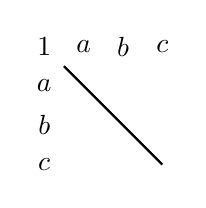
\begin{tikzpicture}[scale=0.5]
			\draw (0,0) node {$1$};
			\draw (1,0) node {$a$};
			\draw (2,0) node {$b$};
			\draw (3,0) node {$c$};
			\draw (0,-1) node {$a$};
			\draw (0,-2) node {$b$};
			\draw (0,-3) node {$c$};
			\draw[thick] (0.5,-0.5) -- (3,-3);
		\end{tikzpicture}
	\end{center}
	Es muss symmetrisch sein. Weil alle Elemente in alle Zeilen und Spalten vorkommen muss, gilt entweder
\end{parts}
\end{proof}
